\documentclass{article}

\usepackage{fancyhdr}
\usepackage{amsmath}
\usepackage{esint}
\usepackage{amsfonts}
\usepackage{amsthm}
\usepackage{amssymb}
\usepackage{caption}
\usepackage{subcaption}
\usepackage{amsbsy}
\usepackage{verbatim}
\usepackage{eucal}
\usepackage{mathrsfs}
\usepackage[hmargin = 1in,vmargin=1in]{geometry}
\usepackage[parfill]{parskip}
\usepackage{listings}
\usepackage{titling}
\usepackage{graphicx}
\graphicspath{ {./images/} }

\usepackage[usenames, dvipsnames]{xcolor}
v\definecolor{dkgray}{rgb}{.4,.4,.4}
\definecolor{dkred}{rgb}{.4,0,0}
\definecolor{dkgreen}{rgb}{0,.4,0}
\definecolor{dkblue}{rgb}{0,0,.4}
 
\definecolor{codegreen}{rgb}{0,0.6,0}
\definecolor{codegray}{rgb}{0.5,0.5,0.5}
\definecolor{codepurple}{rgb}{0.58,0,0.82}
\definecolor{backcolour}{rgb}{0.95,0.95,0.92}
 
\lstdefinestyle{mystyle}{
    backgroundcolor=\color{backcolour},   
    commentstyle=\color{codegreen},
    keywordstyle=\color{magenta},
    numberstyle=\tiny\color{codegray},
    stringstyle=\color{codepurple},
    basicstyle=\ttfamily\footnotesize,
    breakatwhitespace=false,         
    breaklines=true,                 
    captionpos=b,                    
    keepspaces=true,
    numbers=left,                    
    numbersep=5pt,
    showspaces=false,                
    showstringspaces=false,
    showtabs=false,                  
    tabsize=2
}
 
\lstset{style=mystyle}

\setlength{\parskip}{2ex}
\pagestyle{fancy}


\lhead{YSC3217 POSIX}
\chead{Matrix Multiplication Project}
\rhead{Bryan Tan}


\begin{document}
\section{Introduction}
In this report, I document my findings with exploring four more versions of the \texttt{matmul} program: one with $2$ processes, one with $N $ processes, one with $N$ threads, and one using OpenMP. I describe my implementation for each of them before finally showing some plots that compare their runtime across the number of cores used. The code and artefacts are available in the associated folder.
\section{Implementation}
\subsection{2 Processes \texttt{matmul}}
Firstly, we improve upon the naive sequential implementation of \texttt{matmul}. Matrix multiplication as implemented in \texttt{mm\_seq} is inherently parallelizable since accessing the two matrices to perform the multiplication does not change the matrices, so there won't be a race condition. Thus, we can divide the work in half by invoking a new process and having it do one-half of the total multiplications. The only difficulty is handling shared memory - we first construct a ``shared'' matrix to store the result in. Then, when we are done, we copy the matrix into our result matrix $C$, taking care to unmap the memory allocated to the ``shared'' matrix.

As seen in \texttt{mm\_proc.c},
\begin{lstlisting}[language=C]
 void mm ( size_t N, NUMTYPE * A, NUMTYPE * B, NUMTYPE * C) {
  int* T = mmap(NULL, N * N * sizeof (NUMTYPE),
		PROT_READ | PROT_WRITE, MAP_SHARED | MAP_ANONYMOUS,
		-1, 0);
  int child_pid = fork();
  if (child_pid == 0) {
    mm_helper(0, N/2, N, A, B, T);
    exit(0);
  } else {
    mm_helper(N/2, N, N, A, B, T);
  }
  wait(NULL);
  memcpy(C, T, sizeof(NUMTYPE) * N * N);
  munmap(T, N * N * sizeof (NUMTYPE));
}  
\end{lstlisting}
where \texttt{mm\_helper} is simply the initial sequential implementation of matrix multiplication abstracted as a helper function.
\subsection{N-Processes \texttt{matmul}}
When generalizing the above to $N$-processes, the intuition is the same: allocate memory for a ``shared'' matrix, perform the multiplication with $N$ processes, then copy it over to the result matrix. However, an important thing to note is that the dimensions of the $n \times n$ matrix may not be perfectly divisible by $N$. For instance, if we have a $500 \times 500$ matrix, with $16$ processes, $500$ is not perfectly divisible by $16$. So we have to account for this by finding the remainder with the modulo infix operator, and then handling that case specially. Other than that, the implementation is similar: in \texttt{mm\_procn.c}, we have

\begin{lstlisting}[language=C]
  void mm ( size_t N, NUMTYPE * A, NUMTYPE * B, NUMTYPE * C) {
  int* T = mmap(NULL, N * N * sizeof (NUMTYPE),
		PROT_READ | PROT_WRITE, MAP_SHARED | MAP_ANONYMOUS,
		-1, 0);  
  int i = 0; 
  int slice;
  int leftover = N % NUM_PROCESSES;
  if (leftover  == 0) { 
    slice = N/NUM_PROCESSES;
    while (i < NUM_PROCESSES){
      int child_pid = fork();
      if (child_pid == 0){
	mm_helper(i*slice, (i+1)*slice, N, A,B,T);
	exit(0);
      }
      i++;
    }
    while(wait(NULL)>0);
    memcpy(C, T, sizeof(NUMTYPE) * N * N);
    munmap(T, N * N * sizeof (NUMTYPE));
  } else {//account for when N cannot be perfectly divided by NUM_PROCESSES
    slice = (N-leftover)/NUM_PROCESSES;
    while (i< NUM_PROCESSES ){
      int child_pid = fork();
      if (child_pid == 0){
	mm_helper(i*slice, (i+1)*slice, N, A,B,T);
	exit(0);
      }
      i++;
    }
    while(wait(NULL)>0);
    mm_helper(i*slice, (i*slice)+leftover,N,A,B,T);
    memcpy(C, T, sizeof(NUMTYPE) * N * N);
    munmap(T, N * N * sizeof (NUMTYPE));
  }
\end{lstlisting}
\subsection{N-Threads \texttt{matmul}}
Again, the idea for using $N$-threads is very similar to using $N$-processes, except now we don't use shared memory since the threads \emph{do} share memory already. Firstly, we spawn $N$ threads, telling them to perform their share of the matrix multiplication. Then, we \texttt{join} them. As before, special care is taken to account for the remainder since the dimensions of the matrix may not be perfectly divisible by $N$.

In this case, however, we employ the help of a \texttt{lock} to lock the critical section where we calculate the portion of the matrix multiplication that each thread does. The reason for this is because each thread, running in parallel, decides its portion of the matrix multiplication by reading a global variable \texttt{curr\_thread}, and then incrementing it for the next thread. Thus, there is the possibility of a data race since the actions are not atomic. Therefore, we lock this critical section, as shown in \texttt{mm\_threadsn.c}:

\begin{lstlisting}[language=C]
    //lock the critical section; might be instances where these values are changed before the current thread uses them, affecting correctness of the program
  pthread_mutex_lock(&lock);
  int i = curr_thread++;
  int start = i*N/NUM_THREADS;
  int end = (i+1) *N/NUM_THREADS;
  pthread_mutex_unlock(&lock);
  for (int x = start; x < end ; x++) {
    for (unsigned int y = 0 ; y < N ; y++) {
      unsigned int tidx = x + y * N ;
      C[tidx] = 0;
      for (unsigned int d = 0 ; d < N ; d++) {
	C[tidx] += A[d + y * N] * B[x + d * N] ;
      }
    }
  }
\end{lstlisting}

The rest of the code is fairly straightforward.
\subsection{OpenMP \texttt{matmul}}
For OpenMP, we just add in a pre-processing directive \texttt{pragma} to specify that the compiler should use the OpenMP compiler extension to optimize the code by adding in parallelism. Then, when compiling, we tell the compiler that we are using this extension by adding the flag ``-fopenmp'' so that it links properly.  What's interesting is that the pragmas are designed so that even if the compiler does not support them, the program will still yield correct behavior, but without any parallelism.

See: \texttt{mm\_openmp.c}
\begin{lstlisting}{language=C}
  void mm (size_t N, NUMTYPE * A, NUMTYPE * B, NUMTYPE * C) {
  unsigned int x,y,d;
#pragma omp parallel for shared(A,B,C) private(x,y,d)

  for ( x = 0 ; x < N ; x++) {
    for ( y = 0 ; y < N ; y++) {
      unsigned int tidx = x + y * N ;
      NUMTYPE tmp = 0;
      for ( d = 0 ; d < N ; d++) {
	  tmp += A[d + y * N] * B[x + d * N] ;
      }
      C[tidx] = tmp;
    }
  }
}
\end{lstlisting}

Essentially, \texttt{\#pragma omp parallel for} starts a team of threads (whose number is determined at runtime) to delegate portion of the \texttt{for}-loop to. \texttt{shared(A,B,C)} just informs OpenMP what memory is able to be shared, and \texttt{private(x,y,d)} says what is private.

\section{Evaluation}
To generate the plots for this section, just run \texttt{make graphs} from the \texttt{matmul\_process\_and\_threads} directory. Please pardon my amateur-ish attempt at automating it using the Makefile and python scripting. The requirements are that you have \texttt{python3} and \texttt{matplotlib} library for \texttt{python} installed (works for python 2 as well I think but I worked in python 3).

\begin{figure}[!h]
\centering  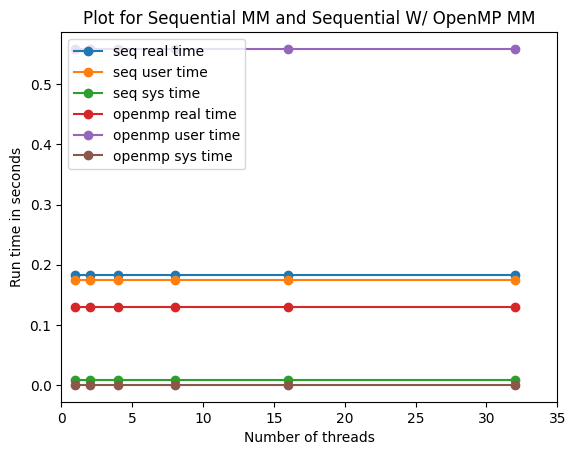
\includegraphics[width=0.5\textwidth]{others}
\label{fig: mm_seq and mm_openmp}
\caption{Run time for mm\_seq and mm\_openmp}
\end{figure}

In figure 1, we simply have a horizontal line for the runtime since sequential matrix multiplication is, well, sequential, and because OpenMP determines at runtime the optimal number of cores, so it is fixed. We see that the OpenMP implementation is significantly faster than the naive sequential one in terms of real time (blue line v.s. red line). However, since OpenMP uses significant multithreading, the user time for OpenMP matrix multiplication (purple line) is very high which signifies the usage of multiple cores and threads.

  \begin{figure}[!h]
  \begin{subfigure}[t]{.5\textwidth}
    \centering    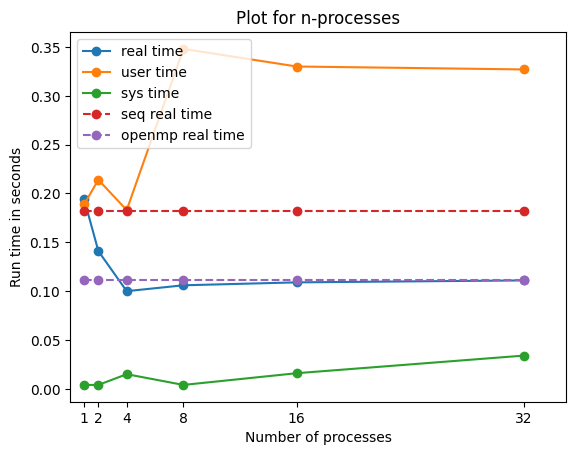
\includegraphics[width=\linewidth]{mm_procn.png}
    \caption {Run time for mm\_procn}
    %\label{fig:draketl}
  \end{subfigure}
  \hfill
  \begin{subfigure}[t]{.5\textwidth}
    \centering
    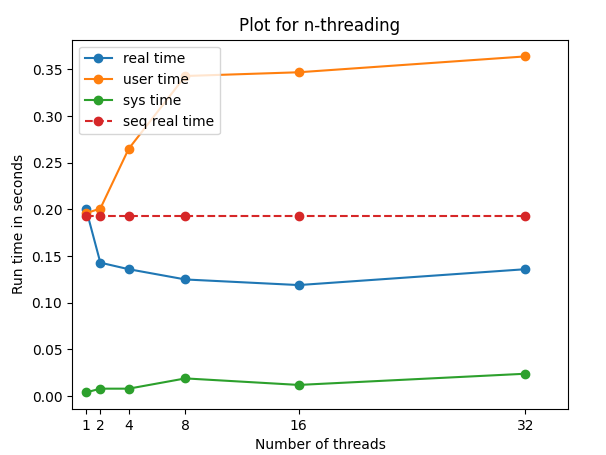
\includegraphics[width=\linewidth]{mm_threadsn.png}
    \caption{Run time for mm\_threadsn}
        %\label{fig:draketr}
  \end{subfigure}
\end{figure}

For \texttt{mm\_procn} and \texttt{mm\_threadsn}, we compare their real, user, and sys times as well. We also overlay the previous sequential and OpenMP real runtimes just for easier comparison. Looking at figures (a) and (b), we see that for both implementations, the real run time (blue line) decreases as more threads are being used (tested on 1,2,4,8,16,32 threads). As one expects, as the number of threads increases, and the real run time decreases, the user time (orange line) increases as the total CPU time is increased since we utilize more of it. We see that the improvements to real runtime stabilizes after around 16 threads, which is probably the upper limit of actual hardware threads available, and after that the threads are just software threads being spawned that don't improve the runtime. We see that both \texttt{mm\_threadsn} and \texttt{mm\_procn} perform comparably to \texttt{OpenMP} after 8 threads, which is wonderful because it means my implementation was almost as efficient.

\end{document}

%%% Local Variables:
%%% mode: latex
%%% TeX-master: t
%%% End:
